% Options for packages loaded elsewhere
\PassOptionsToPackage{unicode}{hyperref}
\PassOptionsToPackage{hyphens}{url}
\PassOptionsToPackage{dvipsnames,svgnames,x11names}{xcolor}
\documentclass[
  10pt,
  fontset=fandol]{ctexart}
\usepackage{xcolor}
\usepackage[margin=16mm]{geometry}
\usepackage{amsmath,amssymb}
\setcounter{secnumdepth}{-\maxdimen} % remove section numbering
\usepackage{iftex}
\ifPDFTeX
  \usepackage[T1]{fontenc}
  \usepackage[utf8]{inputenc}
  \usepackage{textcomp} % provide euro and other symbols
\else % if luatex or xetex
  \usepackage{unicode-math} % this also loads fontspec
  \defaultfontfeatures{Scale=MatchLowercase}
  \defaultfontfeatures[\rmfamily]{Ligatures=TeX,Scale=1}
\fi
\usepackage{lmodern}
\ifPDFTeX\else
  % xetex/luatex font selection
\fi
% Use upquote if available, for straight quotes in verbatim environments
\IfFileExists{upquote.sty}{\usepackage{upquote}}{}
\IfFileExists{microtype.sty}{% use microtype if available
  \usepackage[]{microtype}
  \UseMicrotypeSet[protrusion]{basicmath} % disable protrusion for tt fonts
}{}
\makeatletter
\@ifundefined{KOMAClassName}{% if non-KOMA class
  \IfFileExists{parskip.sty}{%
    \usepackage{parskip}
  }{% else
    \setlength{\parindent}{0pt}
    \setlength{\parskip}{6pt plus 2pt minus 1pt}}
}{% if KOMA class
  \KOMAoptions{parskip=half}}
\makeatother
\usepackage{graphicx}
\makeatletter
\newsavebox\pandoc@box
\newcommand*\pandocbounded[1]{% scales image to fit in text height/width
  \sbox\pandoc@box{#1}%
  \Gscale@div\@tempa{\textheight}{\dimexpr\ht\pandoc@box+\dp\pandoc@box\relax}%
  \Gscale@div\@tempb{\linewidth}{\wd\pandoc@box}%
  \ifdim\@tempb\p@<\@tempa\p@\let\@tempa\@tempb\fi% select the smaller of both
  \ifdim\@tempa\p@<\p@\scalebox{\@tempa}{\usebox\pandoc@box}%
  \else\usebox{\pandoc@box}%
  \fi%
}
% Set default figure placement to htbp
\def\fps@figure{htbp}
\makeatother
\setlength{\emergencystretch}{3em} % prevent overfull lines
\providecommand{\tightlist}{%
  \setlength{\itemsep}{0pt}\setlength{\parskip}{0pt}}
\usepackage{amsmath,amssymb,mathtools,needspace}
\xeCJKDeclareCharClass{CJK}{"2032,"0400->"04FF,"2160->"216B,"2460->"2473,"25A0,"25C7,"25CB,"25CF}
\IfFontExistsTF{Arial Unicode MS}{\xeCJKsetup{AutoFallBack=true}\setCJKfallbackfamilyfont{\CJKrmdefault}{Arial Unicode MS}}{}
\setcounter{secnumdepth}{0}
\setlength{\emergencystretch}{2em}
\allowdisplaybreaks
\usepackage{bookmark}
\IfFileExists{xurl.sty}{\usepackage{xurl}}{} % add URL line breaks if available
\urlstyle{same}
\hypersetup{
  pdftitle={Newton 法的几何解释},
  colorlinks=true,
  linkcolor={Maroon},
  filecolor={Maroon},
  citecolor={Blue},
  urlcolor={Blue},
  pdfcreator={LaTeX via pandoc}}

\title{Newton 法的几何解释}
\author{}
\date{}

\begin{document}
\maketitle

\subsubsection{6.3.2 Newton 法的几何解释}\label{newton-ux6cd5ux7684ux51e0ux4f55ux89e3ux91ca}

对于方程 \(f(x)=0\)，如果 \(f(x)\) 是线性函数，则对它求根是容易的。Newton 法实质上是一种线性化方法，其基本思想是将非线性方程 \(f(x)=0\) 逐步归结为某种线性方程来求解。

设已知方程 \(f(x)=0\) 有近似根 \(x_k\)，将函数 \(f(x)\) 在点 \(x_k\) 展开，有

\[
f(x)\approx f(x_k)+f'(x_k)(x-x_k),
\]

于是方程 \(f(x)=0\) 可近似地表示为

\[
f(x_k)+f'(x_k)(x-x_k)=0.
\tag{6.3.4}
\]

这是个线性方程，记其根为 \(x_{k+1}\)，则 \(x_{k+1}\) 的计算公式就是 Newton 公式（6.3.3）。

Newton 法有明显的几何解释。方程 \(f(x)=0\) 的根 \(x^*\) 可解释为曲线 \(y=f(x)\) 与 \(x\) 轴的交点的横坐标（见图 6.3）。设 \(x_k\) 是根 \(x^*\) 的某个近似值，过曲

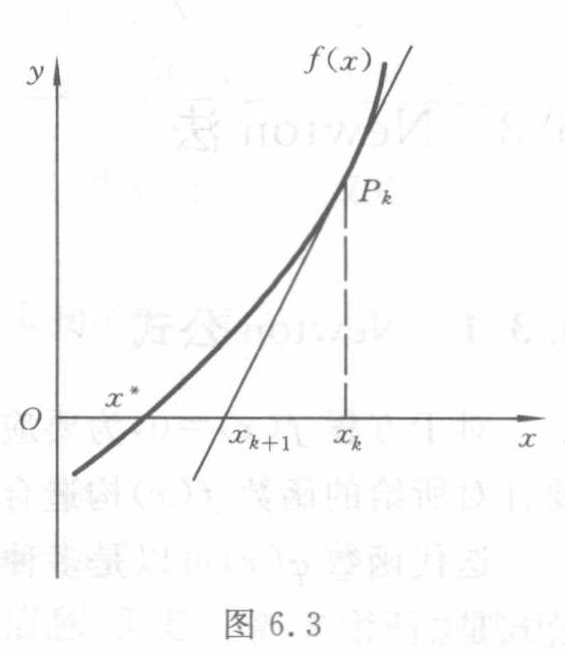
\includegraphics[width=0.85\linewidth,height=\textheight,keepaspectratio,alt={图 6.3 原扫描裁切}]{../assets/ch06/fig-6.3.png}

图 6.3

图意（agent 整理）：曲线 \(f(x)\) 在 \(P_k\) 处的切线与 \(x\) 轴相交，其交点横坐标是 \(x_{k+1}\)。全部标签为 \(x,\allowbreak y,\allowbreak O,\allowbreak x^*,\allowbreak x_{k+1},\allowbreak x_k,\allowbreak P_k,\allowbreak f(x)\)。

\href{../../source-images/pdf-164.jpeg}{原页}

线 \(y=f(x)\) 上横坐标为 \(x_k\) 的点 \(P_k\) 引切线，并将该切线与 \(x\) 轴的交点的横坐标 \(x_{k+1}\) 作为 \(x^*\) 的新的近似值。注意到切线方程为

\[
y=f(x_k)+f'(x_k)(x-x_k).
\]

这样求得的值 \(x_{k+1}\) 必满足式（6.3.4），从而就是 Newton 公式（6.3.3）的计算结果。由于这种几何背景，Newton 法亦称切线法。

\end{document}
